\chapter*{Revisión sistemática de la literatura}\label{cap:revisionLiteratura}

\section*{1. Construcción de la bitácora}
\addcontentsline{toc}{section}{Construcción de la bitácora}\label{sec:bitacora}

En búsqueda de una base teórica para la elección de una tecnología de virtualización basada en contenedores, 
se realizó una revisión del estado del arte. Esta revisión se completó en diferentes etapas:

\subsection*{1.1 Planeación}
\addcontentsline{toc}{subsection}{Planeación}\label{subsec:planeacion}

Esta etapa consistió en establecer el propósito general que se buscaba alcanzar con el SMS (\textit{Systematic Mapping Study}). 
A su vez, definió aspectos como objetivos, preguntas de investigación y métricas. Para ello, se siguió el modelo 
Objetivo-Pregunta-Métrica (\textit{Goal-Question-Metric}, GQM). A continuación, se definen los objetivos del SMS aplicado 
a las tecnologías de virtualización basadas en contenedores.

\subsubsection*{1.1.1 Definición de metas para el SMS}
\addcontentsline{toc}{subsubsection}{Definición de metas para el SMS}\label{subsubsec:metasSMS}

\begin{table}[H]
    \centering
    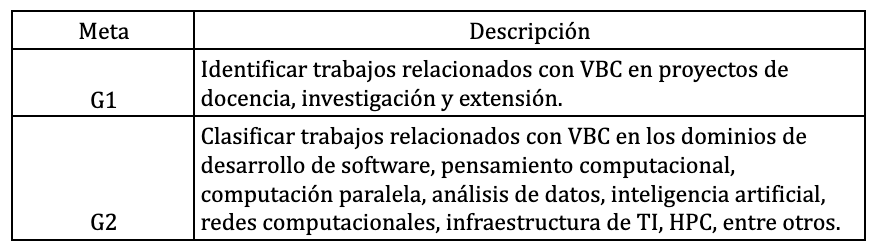
\includegraphics[width=\textwidth] {tablas-images/cp2/definicionMetas.png}
    \caption{Definición de metas del SMS}\label{tab:tabla-metas}
\end{table}

\subsubsection*{1.1.2 Definición de preguntas de investigación}
\addcontentsline{toc}{subsubsection}{Definición de preguntas de investigación}\label{subsubsec:preguntasInvestigacion}

\begin{table}[H]
    \centering
    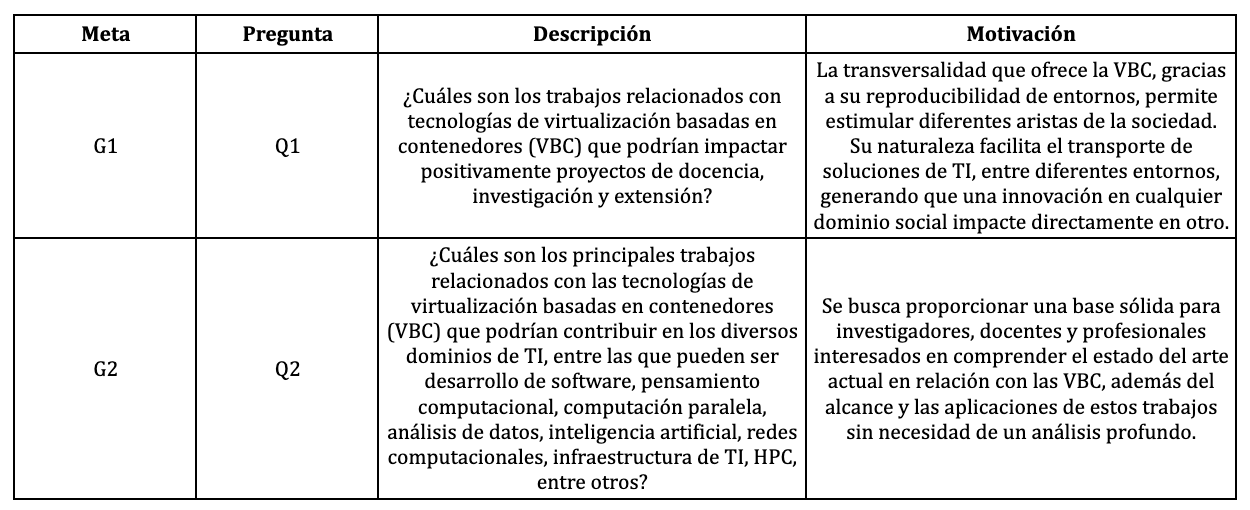
\includegraphics[width=\textwidth] {tablas-images/cp2/preguntasInvestigacion.png}
    \caption{Definición de preguntas de investigación del SMS}\label{tab:tabla-preguntas}
\end{table}

\subsubsection*{1.1.3 Definición de métricas}
\addcontentsline{toc}{subsubsection}{Definición de métricas}\label{subsubsec:metricasSMS}

\begin{figure}[H]
    \centering
    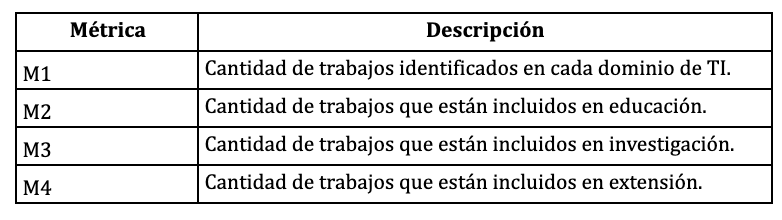
\includegraphics[width=\textwidth] {tablas-images/cp2/definicionMetricas.png}
    \caption{Definición de métricas del SMS}\label{fig:tabla-metricas}
\end{figure}

\section*{2. Búsqueda de estudios}
\addcontentsline{toc}{section}{Búsqueda de estudios}\label{sec:busquedaEstudios}

Esta etapa comprendió las siguientes secciones: 
\begin{enumerate}
  \item Estrategia de búsqueda, ya sea independiente o combinada;
  \item Identificación general de estudios;
  \item Selección; y finalmente,
  \item Selección de estudios para incluir en el SMS.\end{enumerate}

\subsection*{2.1 Estrategia de búsqueda}
\addcontentsline{toc}{subsection}{Estrategia de búsqueda}\label{subsec:estrategiaBusqueda}

Este trabajo combinó las estrategias de búsqueda en bases de datos y búsqueda en bola de nieve. 
Para la estrategia de búsqueda en bases de datos, se seleccionaron las siguientes bases de datos: ACM, IEEE Xplore, Springer, Taylor \& Francis y Science Direct.

\subsection*{2.2 Búsqueda en bases de datos}
\addcontentsline{toc}{subsection}{Búsqueda en bases de datos}\label{subsec:busquedaBasesDatos}
Se seleccionaron las siguientes bases de datos para este propósito: ACM, IEEE Xplore, Springer, Taylor \& Francis y Science Direct.

\subsubsection*{2.2.1 Identificación de estudios mediante búsqueda en bases de datos}
\addcontentsline{toc}{subsubsection}{Identificación de estudios mediante búsqueda en bases de datos}\label{subsubsec:identificacionEstudios}
En esta etapa del proceso fue necesario establecer las palabras clave que serían útiles en las cadenas de búsqueda para cada una de las bases de datos seleccionadas. 
Los términos consideran los elementos identificados en la etapa de planificación, para lo cual también se utilizó el modelo PICOC como guía metodológica.

\begin{table}[H]
    \centering
    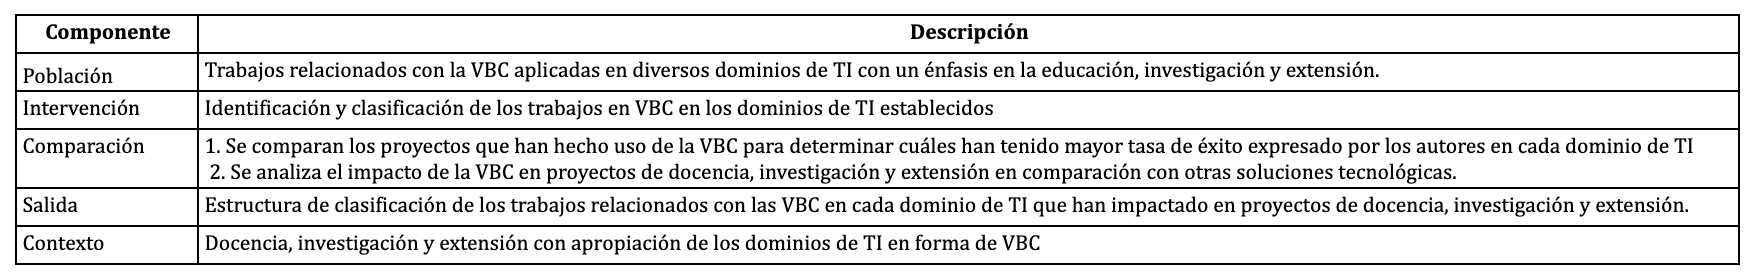
\includegraphics[width=\textwidth] {tablas-images/cp2/modelo-PICOC.png}
    \caption{Modelo PICOC}\label{tab:tabla-PICOC}
\end{table}
\begin{table}[H]
    \centering
    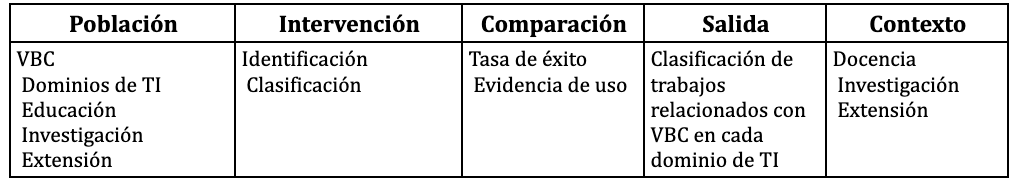
\includegraphics[width=\textwidth] {tablas-images/cp2/keywords-PICOC.png}
    \caption{Palabras clave identificadas usando el modelo PICOC}\label{tab:tabla-keywords-PICOC}
\end{table}
\begin{table}[H]
    \centering
    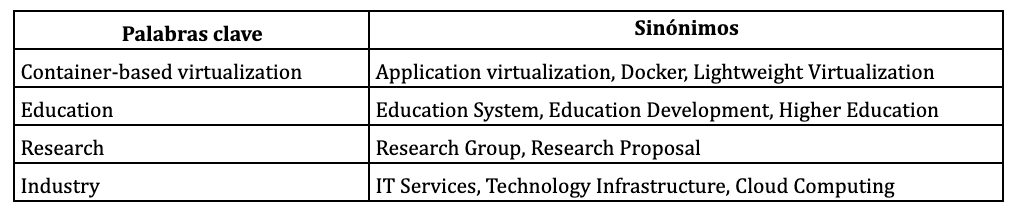
\includegraphics[width=\textwidth] {tablas-images/cp2/keywords.png}
    \caption{Palabras clave para la búsqueda en base de datos}\label{tab:tabla-keywords}
\end{table}
\begin{table}[H]
    \centering
    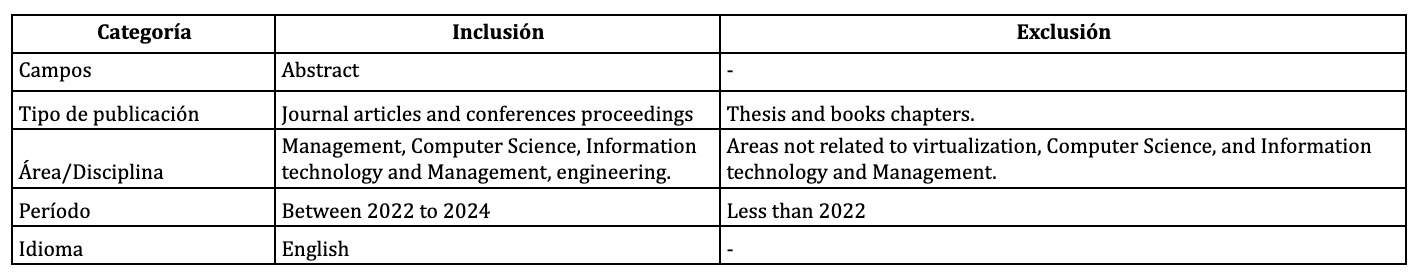
\includegraphics[width=\textwidth] {tablas-images/cp2/criterios.png}
    \caption{Criterios de Inclusión/Exclusión}\label{tab:tabla-criterios}
\end{table}

\subsubsection*{2.2.1.1 Búsqueda en bases de datos}
\addcontentsline{toc}{paragraph}{2.2.1.1 Búsqueda en bases de datos}\label{par:busquedaBasesDatos}

\begin{tcolorbox}[
  colback=gray!5, 
  colframe=black!60, 
  title=Cadena de búsqueda en ACM para educación, 
  fonttitle=\bfseries, 
  sharp corners=south
]
\scriptsize % o \footnotesize, \tiny según lo pequeño que lo quieras
\begin{verbatim}
(Title:("Container-based virtualization" OR "Application virtualization" OR "Docker" OR 
"Lightweight Virtualization") AND Title:("Education" OR "Education System" 
OR "Education Development" OR "Higher Education") ) 

OR

(Abstract:("Container-based virtualization" OR "Application virtualization" OR "Docker"
 OR "Lightweight Virtualization") AND Abstract:("Education" OR "Education System" 
 OR "Education Development" OR "Higher Education") )

OR

(Keyword:("Container-based virtualization" OR "Application virtualization" OR "Docker" OR 
"Lightweight Virtualization")
AND Keyword:("Education" OR "Education System" OR "Education Development" 
OR "Higher Education"))
\end{verbatim}
\end{tcolorbox}

\begin{tcolorbox}[
  colback=gray!5, 
  colframe=black!60, 
  title=Cadena de búsqueda en ACM para investigación, 
  fonttitle=\bfseries, 
  sharp corners=south
]
\scriptsize % puedes usar \tiny para hacerlo aún más pequeño
\begin{verbatim}
(Title:("Container-based virtualization" OR "Application virtualization" OR "Docker" OR 
"Lightweight Virtualization") AND Title:("Research" OR "Research Group" OR 
"Research Proposal"))

OR

(Abstract:("Container-based virtualization" OR "Application virtualization" OR "Docker" OR 
"Lightweight Virtualization") AND Abstract:("Research" OR "Research Group" OR 
"Research Proposal"))

OR

(Keyword:("Container-based virtualization" OR "Application virtualization" OR "Docker" OR 
"Lightweight Virtualization") AND Keyword:("Research" OR "Research Group" OR 
"Research Proposal"))
\end{verbatim}
\end{tcolorbox}

\begin{tcolorbox}[
  colback=gray!5, 
  colframe=black!60, 
  title=Cadena de búsqueda en ACM para industria, 
  fonttitle=\bfseries, 
  sharp corners=south
]
\scriptsize % puedes usar \tiny para hacerlo aún más pequeño
\begin{verbatim}
(Title:("Container-based virtualization" OR "Application virtualization" OR "Docker" OR 
"Lightweight Virtualization") AND Title:("Industry" OR “IT Services” OR 
“Technology Infrastructure” OR “Cloud Computing”) ) 

OR

(Abstract:("Container-based virtualization" OR "Application virtualization" OR "Docker" 
OR "Lightweight Virtualization") AND Abstract:("Industry" OR “IT Services” OR 
“Technology Infrastructure” OR “Cloud Computing”) )

OR

(Keyword:("Container-based virtualization" OR "Application virtualization" OR "Docker" 
OR "Lightweight Virtualization")
AND Keyword:("Industry" OR “IT Services” OR “Technology Infrastructure” 
OR “Cloud Computing”))

\end{verbatim}
\end{tcolorbox}

\begin{tcolorbox}[
  colback=gray!5, 
  colframe=black!60, 
  title=Cadena de búsqueda en IEE para educación, 
  fonttitle=\bfseries, 
  sharp corners=south
]
\scriptsize % puedes usar \tiny para hacerlo aún más pequeño
\begin{verbatim}
(("Abstract":"Container-based virtualization" OR "Abstract":"Application virtualization" 
OR "Abstract":"Docker" OR "Abstract":"Lightweight Virtualization") AND ("Abstract":"Education" 
OR "Abstract":"Education System" OR "Abstract":"Education Development”  OR 
"Abstract":"Higher Education”)) 

OR (("Publication Title":"Container-based virtualization" OR "Publication 
Title":"Application virtualization" 
OR "Publication Title":"Docker" OR "Publication Title":"Lightweight Virtualization") 
AND ("Publication Title":"Education" 
OR "Publication Title":"Education System" OR "Publication Title":"Education Development”  
OR "Publication Title":"Higher Education” ))

OR (("Author Keywords":"Container-based virtualization" OR 
"Author Keywords":"Application virtualization" OR 
"Author Keywords":"Docker" OR "Author Keywords":"Lightweight Virtualization") AND 
("Author Keywords":"Education" 
OR "Author Keywords":"Education System" OR "Author Keywords":"Education Development”  
OR "Author Keywords":"Higher Education”))
\end{verbatim}
\end{tcolorbox}


\begin{tcolorbox}[
  colback=gray!5, 
  colframe=black!60, 
  title=Cadena de búsqueda en IEE para investigación, 
  fonttitle=\bfseries, 
  sharp corners=south
]
\scriptsize % puedes usar \tiny para hacerlo aún más pequeño
\begin{verbatim}
(("Abstract":"Container-based virtualization" OR "Abstract":"Application virtualization" 
OR "Abstract":"Docker" OR "Abstract":"Lightweight Virtualization") AND 
("Abstract":"Research Group" OR "Abstract":"Research Proposal")) 

OR (("Publication Title":"Container-based virtualization" OR 
"Publication Title":"Application virtualization" OR "Publication Title":"Docker" OR 
"Publication Title":"Lightweight Virtualization") AND 
("Publication Title":"Research Group" OR "Publication Title":"Research Proposal" ))

OR (("Author Keywords":"Container-based virtualization" OR 
"Author Keywords":"Application virtualization" OR "Author Keywords":"Docker" OR 
"Author Keywords":"Lightweight Virtualization") AND 
("Author Keywords":"Research Group" OR "Author Keywords":"Research Proposal"))
\end{verbatim}
\end{tcolorbox}

\begin{tcolorbox}[
  colback=gray!5, 
  colframe=black!60, 
  title=Cadena de búsqueda en IEE para industria, 
  fonttitle=\bfseries, 
  sharp corners=south
]
\scriptsize % puedes usar \tiny para hacerlo aún más pequeño
\begin{verbatim}
(("Abstract":"Container-based virtualization" OR "Abstract":"Application virtualization" 
OR "Abstract":"Docker" OR "Abstract":"Lightweight Virtualization") AND 
("Abstract":"Industry" OR "Abstract":"IT Services" OR 
"Abstract":"Technology Infrastructure" OR "Abstract":"Cloud Computing")) 

OR (("Publication Title":"Container-based virtualization" OR 
"Publication Title":"Application virtualization" 
OR "Publication Title":"Docker" OR "Publication Title":"Lightweight Virtualization") AND 
("Publication Title":"Industry" OR "Publication Title":"IT Services" OR 
"Publication Title":"Technology Infrastructure" OR "Publication Title":"Cloud Computing"))

OR (("Author Keywords":"Container-based virtualization" OR 
"Author Keywords":"Application virtualization" OR "Author Keywords":"Docker" OR 
"Author Keywords":"Lightweight Virtualization") AND ("Author Keywords":"Industry" OR 
"Author Keywords":"IT Services" OR "Author Keywords":"Technology Infrastructure" OR 
"Author Keywords":"Cloud Computing"))
\end{verbatim}
\end{tcolorbox}

\begin{tcolorbox}[
  colback=gray!5, 
  colframe=black!60, 
  title=Cadena de búsqueda en Springer para educación, 
  fonttitle=\bfseries, 
  sharp corners=south
]
\scriptsize % puedes usar \tiny para hacerlo aún más pequeño
\begin{verbatim}
(title:("Container-based virtualization" OR "Application virtualization" OR 
"Docker" OR "Lightweight Virtualization") AND title:("Education" OR 
"Education System" OR "Education Development" OR "Higher Education"))

OR

(abstract:("Container-based virtualization" OR "Application virtualization" OR 
"Docker" OR "Lightweight Virtualization") AND abstract:("Education" OR 
"Education System" OR "Education Development" OR "Higher Education"))

OR 

(keyword:("Container-based virtualization" OR "Application virtualization" OR 
"Docker" OR "Lightweight Virtualization") AND keyword:("Education" OR 
"Education System" OR "Education Development" OR "Higher Education"))

\end{verbatim}
\end{tcolorbox}

\begin{tcolorbox}[
  colback=gray!5, 
  colframe=black!60, 
  title=Cadena de búsqueda en Springer para investigación, 
  fonttitle=\bfseries, 
  sharp corners=south
]
\scriptsize % puedes usar \tiny para hacerlo aún más pequeño
\begin{verbatim}
(title:("Container-based virtualization" OR "Application virtualization" OR 
"Docker" OR "Lightweight Virtualization") AND title:("research" OR 
"Research Group" OR "Research Proposal"))

OR

(abstract:("Container-based virtualization" OR "Application virtualization" 
OR "Docker" OR "Lightweight Virtualization") AND abstract:("research" 
OR "Research Group" OR "Research Proposal"))

OR 

(keyword:("Container-based virtualization" OR "Application virtualization"
 OR "Docker" OR "Lightweight Virtualization") AND keyword:("research" OR 
 "Research Group" OR "Research Proposal"))

\end{verbatim}
\end{tcolorbox}

\begin{tcolorbox}[
  colback=gray!5, 
  colframe=black!60, 
  title=Cadena de búsqueda en Springer para industria, 
  fonttitle=\bfseries, 
  sharp corners=south
]
\scriptsize % puedes usar \tiny para hacerlo aún más pequeño
\begin{verbatim}
(title:("Container-based virtualization" OR "Application virtualization"
 OR "Docker" OR "Lightweight Virtualization") AND title:("Industry" OR 
 “IT Services” OR “Technology Infrastructure” OR “Cloud Computing”))

OR

(abstract:("Container-based virtualization" OR "Application virtualization" 
OR "Docker" OR "Lightweight Virtualization") AND abstract:("Industry" OR 
“IT Services” OR “Technology Infrastructure” OR “Cloud Computing”))

OR 

(keyword:("Container-based virtualization" OR "Application virtualization"
 OR "Docker" OR "Lightweight Virtualization") AND keyword:("Industry" 
 OR “IT Services” OR “Technology Infrastructure” OR “Cloud Computing”))

\end{verbatim}
\end{tcolorbox}

\begin{tcolorbox}[
  colback=gray!5, 
  colframe=black!60, 
  title=Cadena de búsqueda en Science Direct para educación, 
  fonttitle=\bfseries, 
  sharp corners=south
]
\scriptsize % puedes usar \tiny para hacerlo aún más pequeño
\begin{verbatim}
("Container-based virtualization" OR "Application virtualization" 
OR "Docker" OR "Lightweight Virtualization")  AND ("Education" OR 
"Education System" OR "Education Development" OR "Higher Education")
\end{verbatim}
\end{tcolorbox}


\begin{tcolorbox}[
  colback=gray!5, 
  colframe=black!60, 
  title=Cadena de búsqueda en Science Direct para investigación, 
  fonttitle=\bfseries, 
  sharp corners=south
]
\scriptsize % puedes usar \tiny para hacerlo aún más pequeño
\begin{verbatim}
("Container-based virtualization" OR "Application virtualization" OR 
"Docker" OR "Lightweight Virtualization")  AND ("Research" OR 
"Research Group" OR "Research Proposal")
\end{verbatim}
\end{tcolorbox}

\begin{tcolorbox}[
  colback=gray!5, 
  colframe=black!60, 
  title=Cadena de búsqueda en Science Direct para industria, 
  fonttitle=\bfseries, 
  sharp corners=south
]
\scriptsize % puedes usar \tiny para hacerlo aún más pequeño
\begin{verbatim}
("Container-based virtualization" OR "Application virtualization" OR "Docker" OR 
"Lightweight Virtualization")  AND 
(“Industry” OR "IT Services" OR "Technology Infrastructure" OR "Cloud Computing")
\end{verbatim}
\end{tcolorbox}

\begin{tcolorbox}[
  colback=gray!5, 
  colframe=black!60, 
  title=Cadena de búsqueda en Taylor \& Francis para educación, 
  fonttitle=\bfseries, 
  sharp corners=south
]
\scriptsize % puedes usar \tiny para hacerlo aún más pequeño
\begin{verbatim}
("Application virtualization" OR "Docker" OR "Lightweight Virtualization" OR "Docker Container")   
AND   
("Education System" OR "Education Sector" OR "Education Development" OR "Higher Education")
\end{verbatim}
\end{tcolorbox}

\begin{tcolorbox}[
  colback=gray!5, 
  colframe=black!60, 
  title=Cadena de búsqueda en Taylor \& Francis para investigación, 
  fonttitle=\bfseries, 
  sharp corners=south
]
\scriptsize % puedes usar \tiny para hacerlo aún más pequeño
\begin{verbatim}
("Application virtualization" OR "Docker" OR "Lightweight Virtualization" OR "Docker Container")
AND   
("Specific Research Areas" OR "Research Group" OR "Research Proposal" OR "Research and Development")
\end{verbatim}
\end{tcolorbox}

\begin{tcolorbox}[
  colback=gray!5, 
  colframe=black!60, 
  title=Cadena de búsqueda en Taylor \& Francis para industria, 
  fonttitle=\bfseries, 
  sharp corners=south
]
\scriptsize % puedes usar \tiny para hacerlo aún más pequeño
\begin{verbatim}
("Application virtualization" OR "Docker" OR "Lightweight Virtualization" OR "Docker Container")  
AND 
(“Industry” OR "IT Services" OR "Technology Infrastructure" OR "Cloud Computing")
\end{verbatim}
\end{tcolorbox}

\subsubsection*{2.2.2 Resumen de la búsqueda en bases de datos sin criterios de inclusión/exclusión}
\addcontentsline{toc}{subsubsection}{Resumen de la búsqueda en bases de datos sin criterios de inclusión/exclusión}\label{subsubsec:resumenBusqueda}
Este es el resultado antes de aplicar criterios de exclusión

\begin{table}[H]
    \centering
    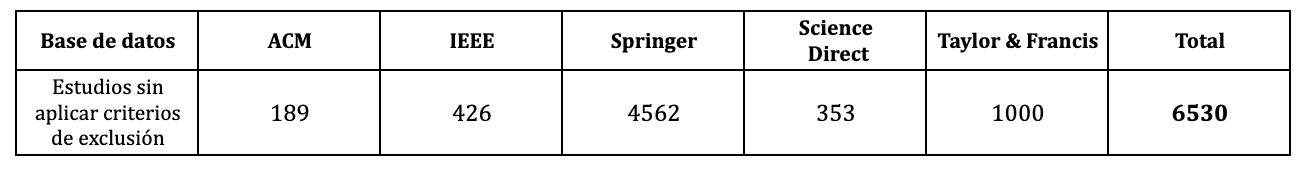
\includegraphics[width=\textwidth] {tablas-images/cp2/resumen-sin-criterios.png}
    \caption{Resumen de la búsqueda en bases de datos sin criterios de inclusión/exclusión}\label{tab:tabla-resumen-sin-criterios}
\end{table}
\begin{figure}[H]
    \centering
    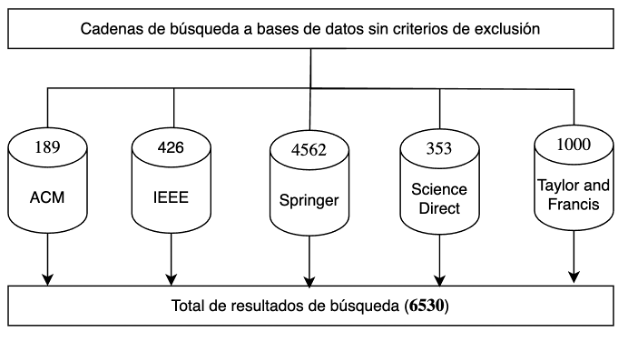
\includegraphics[scale=0.9]{tablas-images/cp2/bases-sin-criterio.png}
    \caption{Diagrama de búsqueda en bases de datos}\label{fig:tabla-resumen-busqueda}
\end{figure}

\subsubsection*{2.2.3	Aplicación de criterios de exclusión de las bases de datos}
Esta búsqueda se realizó considerando los criterios de exclusión e inclusión definidos previamente.

Las cadena de búsqueda son exactamente iguales que antes, este punto se diferencia por la aplicación de 
filtros. Para ver las capturas de pantalla veáse el apéndice B sección 2.

\subsection*{2.3 Resumen de la búsqueda en bases de datos con criterios de inclusión/exclusión}
\addcontentsline{toc}{subsection}{Resumen de la búsqueda en bases de datos con
    criterios de inclusión/exclusión}\label{subsec:resumenBusquedaCriterios}

\begin{table}[H]
\centering
\scriptsize
\setlength{\tabcolsep}{4pt}
\renewcommand{\arraystretch}{1.1}
\begin{tabular}{|l|c|c|c|c|c|c|}
\hline
\textbf{Bases de datos} & \textbf{ACM} & \textbf{IEEE} & \textbf{Springer} & \textbf{Science Direct} & \textbf{Taylor \& Francis} & \textbf{Total} \\
\hline
Con criterios aplicados & 48 & 134 & 592 & 46 & 156 & 976 \\
\hline
\end{tabular}
\caption{Resumen de la búsqueda en bases de datos con criterios de inclusión/exclusión}\label{tab:resumen-busqueda}
\end{table}
\begin{figure}[H]
    \centering
    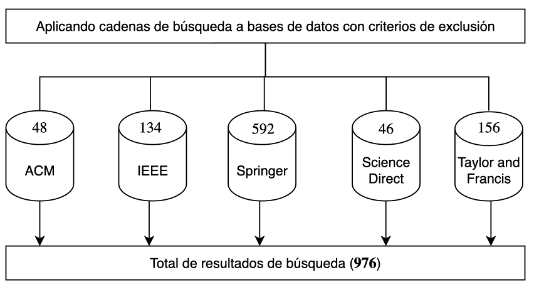
\includegraphics[width=\textwidth] {tablas-images/cp2/bases-con-criterio.png}
    \caption{Resumen de la búsqueda en bases de datos con criterios de inclusión/exclusión}\label{fig:tabla-resumen-busqueda-con-criterio}
\end{figure}

\section*{3 Eliminación de duplicados}
\addcontentsline{toc}{section}{Eliminación de duplicados}\label{sec:eliminacionDuplicados}
La eliminación de duplicados se realizó haciendo uso de la herramienta de gestión de referencias Mendeley. Luego de obtener los artículos se agregaron a Mendeley y esta herramienta se encargó de eliminar duplicados. En este punto se eliminaron 274 artículos duplicados.

\section*{4 Priorización de estudios}
\addcontentsline{toc}{section}{Priorización de estudios}\label{sec:priorizacionEstudios}

Luego de la selección inicial de los artículos, se procedió a revisar el \textit{title}, \textit{abstract} y \textit{keywords} de cada uno. Como resultado de esta revisión, se generaron métricas de calidad para cada artículo, con el fin de priorizar aquellos más relevantes para la investigación. Las métricas utilizadas fueron las siguientes:

\begin{itemize}
    \item \textbf{SCI} (Science Citation Index)
    \item \textbf{CVI} (Core Value Index)
    \item \textbf{IRRQ} (Index Relation Research Question)
\end{itemize}

Este proceso inició con un total de 771 artículos, los cuales fueron evaluados según su alineamiento con los objetivos de la investigación. La evaluación temática permitió identificar un total de 110 artículos con una relación directa con el enfoque planteado.

\section*{5 Estrategia de búsqueda usando bola de nieve}
\addcontentsline{toc}{section}{Estrategia de búsqueda usando bola de nieve}\label{sec:bolaDeNieve}

En esta etapa, se seleccionó el primer cuartil según el índice \textbf{IRRQ}, lo que resultó en un total de 24 artículos. Adicionalmente, se incluyeron dos artículos por criterio de inclusión directa, estableciendo así una línea base de \textbf{26 artículos}. 

Sobre esta base, se aplicó la estrategia de \textit{bola de nieve} en ambas direcciones: hacia adelante y hacia atrás. Como resultado, se obtuvieron \textbf{87 artículos} mediante la técnica hacia atrás y \textbf{495 artículos} mediante la técnica hacia adelante. 

Esto definió un nuevo conjunto de artículos para un proceso de selección adicional (\textit{screening}). En esta fase, se eliminaron \textbf{14 duplicados} y \textbf{452 artículos} fueron descartados por no estar alineados con la investigación. 

Finalmente, se obtuvo un total de \textbf{116 artículos} mediante esta estrategia de búsqueda ampliada.

\section*{6 Diagrama de búsqueda}
\addcontentsline{toc}{section}{Diagrama de búsqueda}\label{sec:diagramaBusqueda}

\subsection*{6.1 Usando cadenas de búsqueda}
\addcontentsline{toc}{subsection}{Usando cadenas de búsqueda}\label{subsec:cadenaBusqueda}
\begin{table}[H]
    \centering
    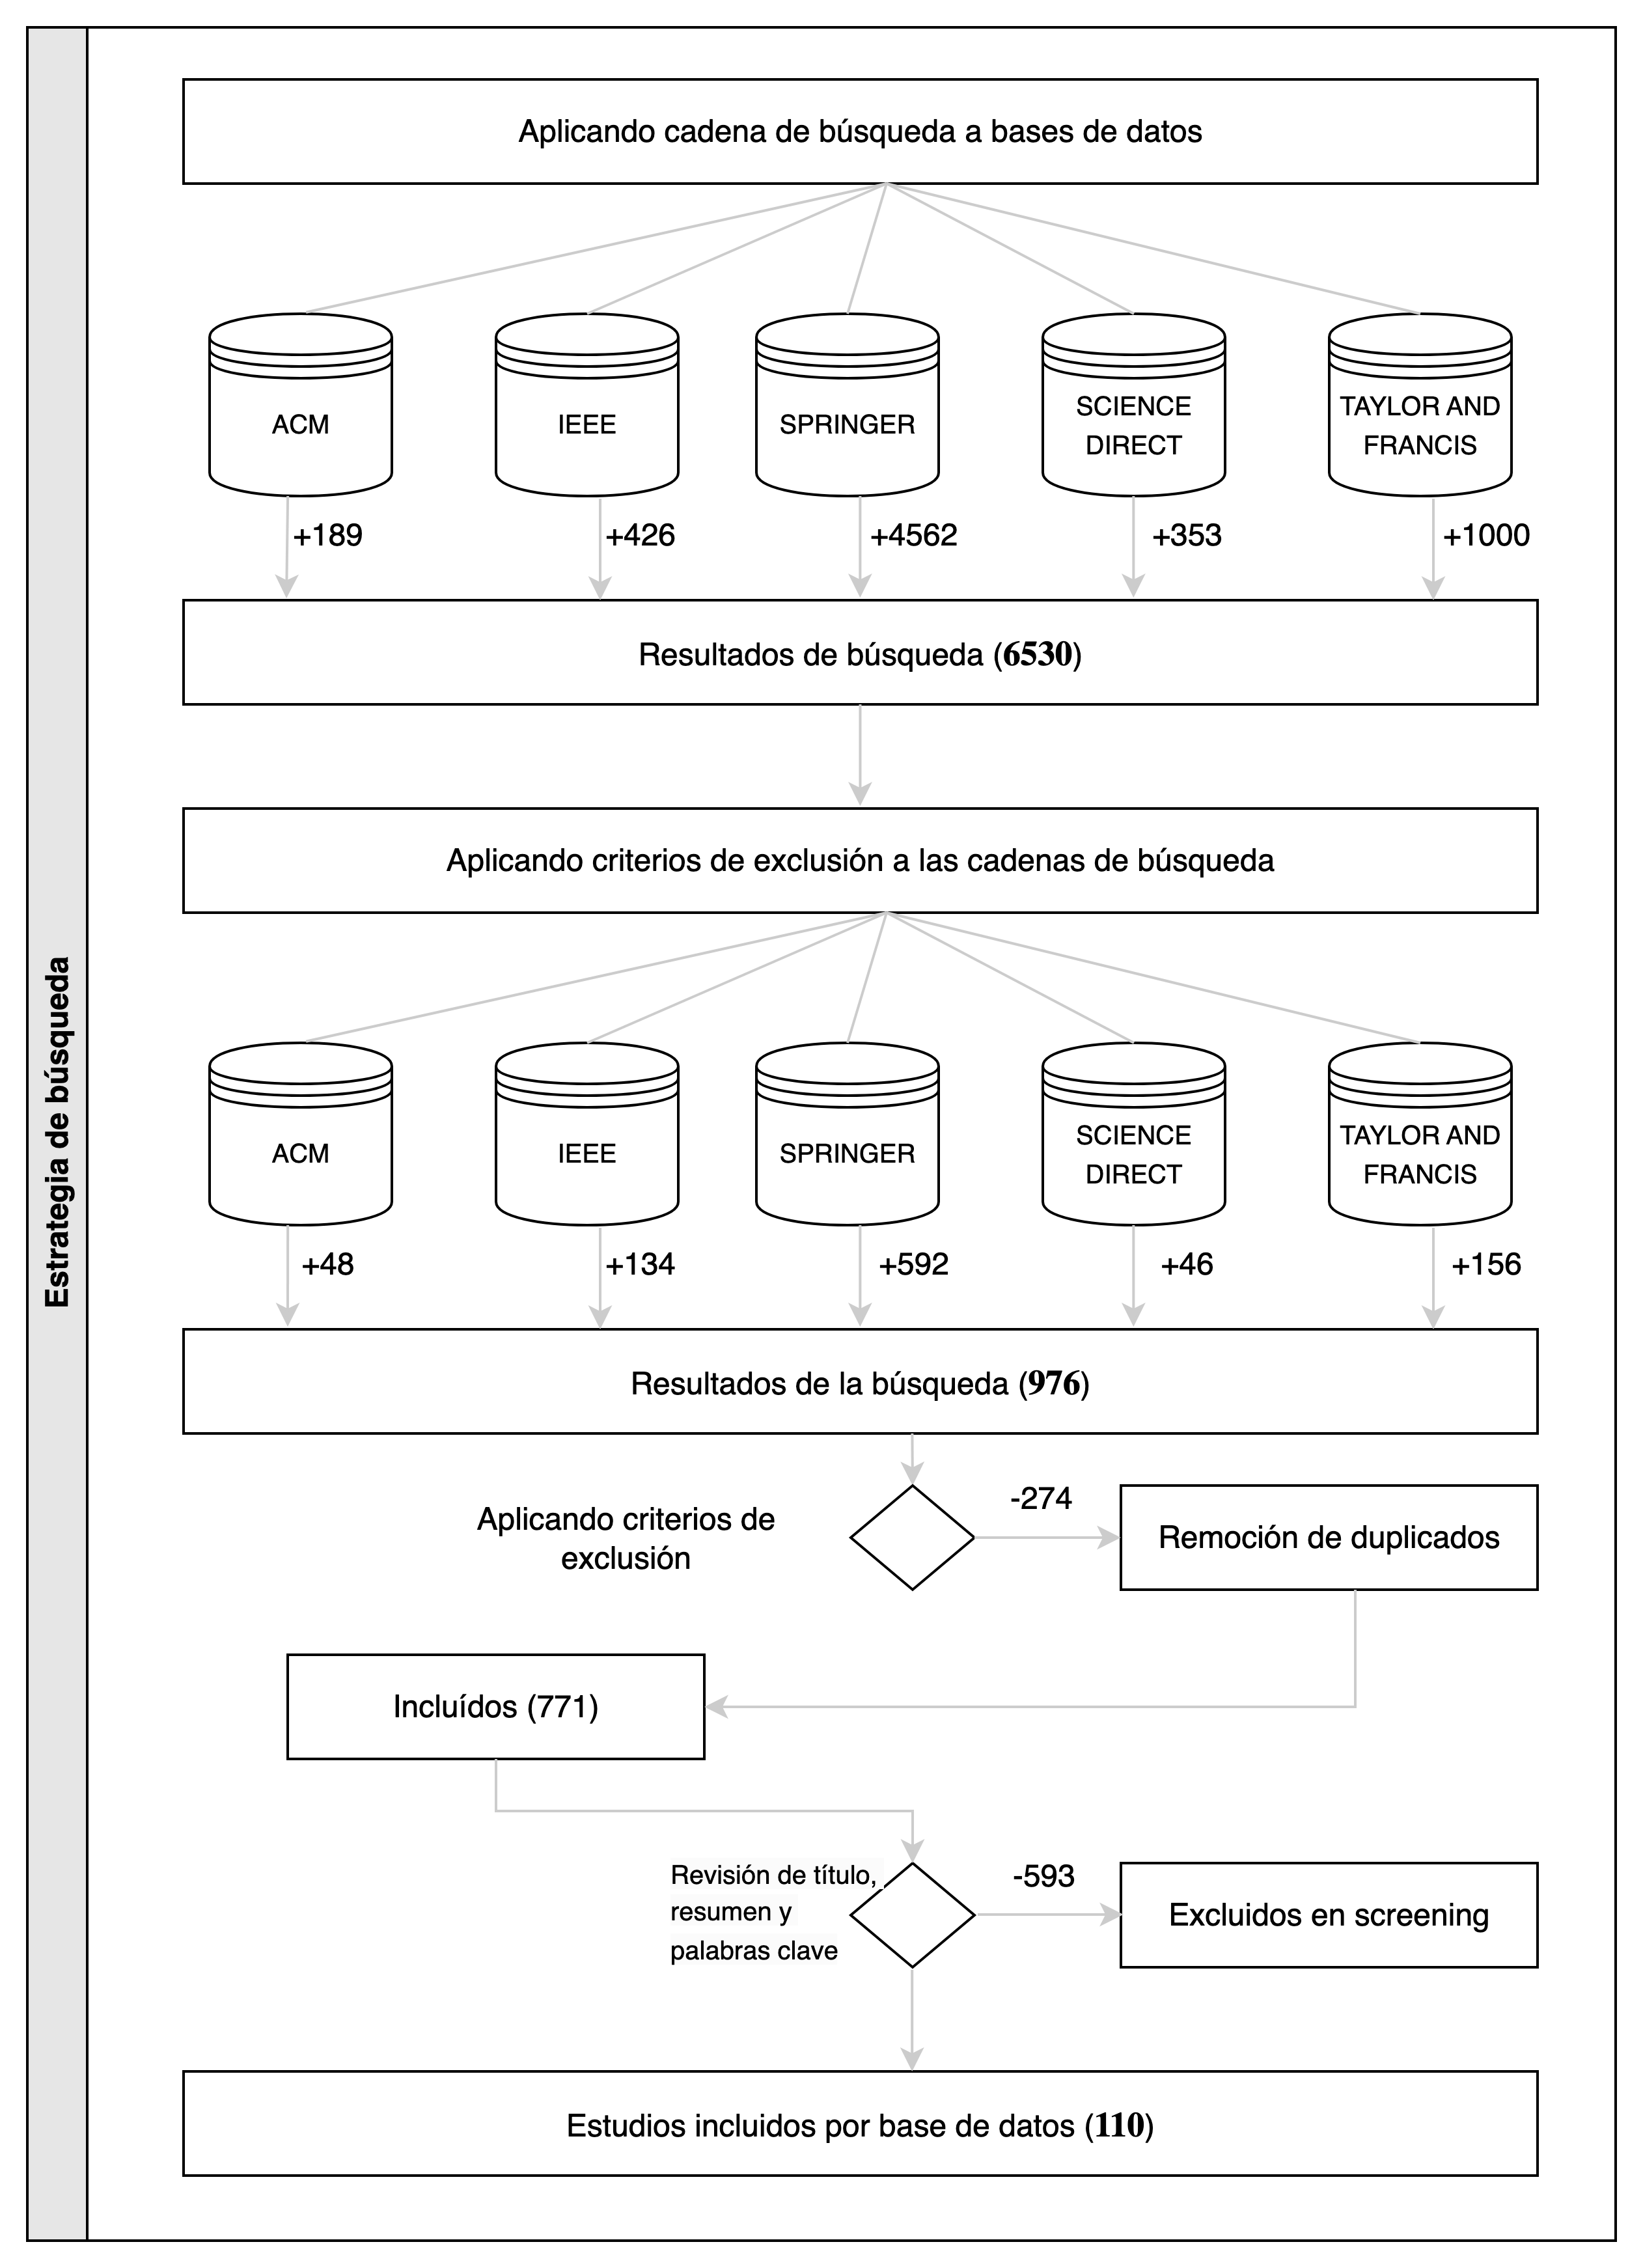
\includegraphics[scale=0.13]{tablas-images/cp2/diagrama-cadena-busqueda.png}
    \caption{Diagrama de la cadena de búsqueda}\label{tab:tabla-diagrama-cadena-busqueda}
\end{table}

\subsection*{6.2 Usando bola de nieve}
\addcontentsline{toc}{subsection}{Usando bola de nieve}\label{subsec:bolaNieveBusqueda}
\begin{table}[H]
    \centering
    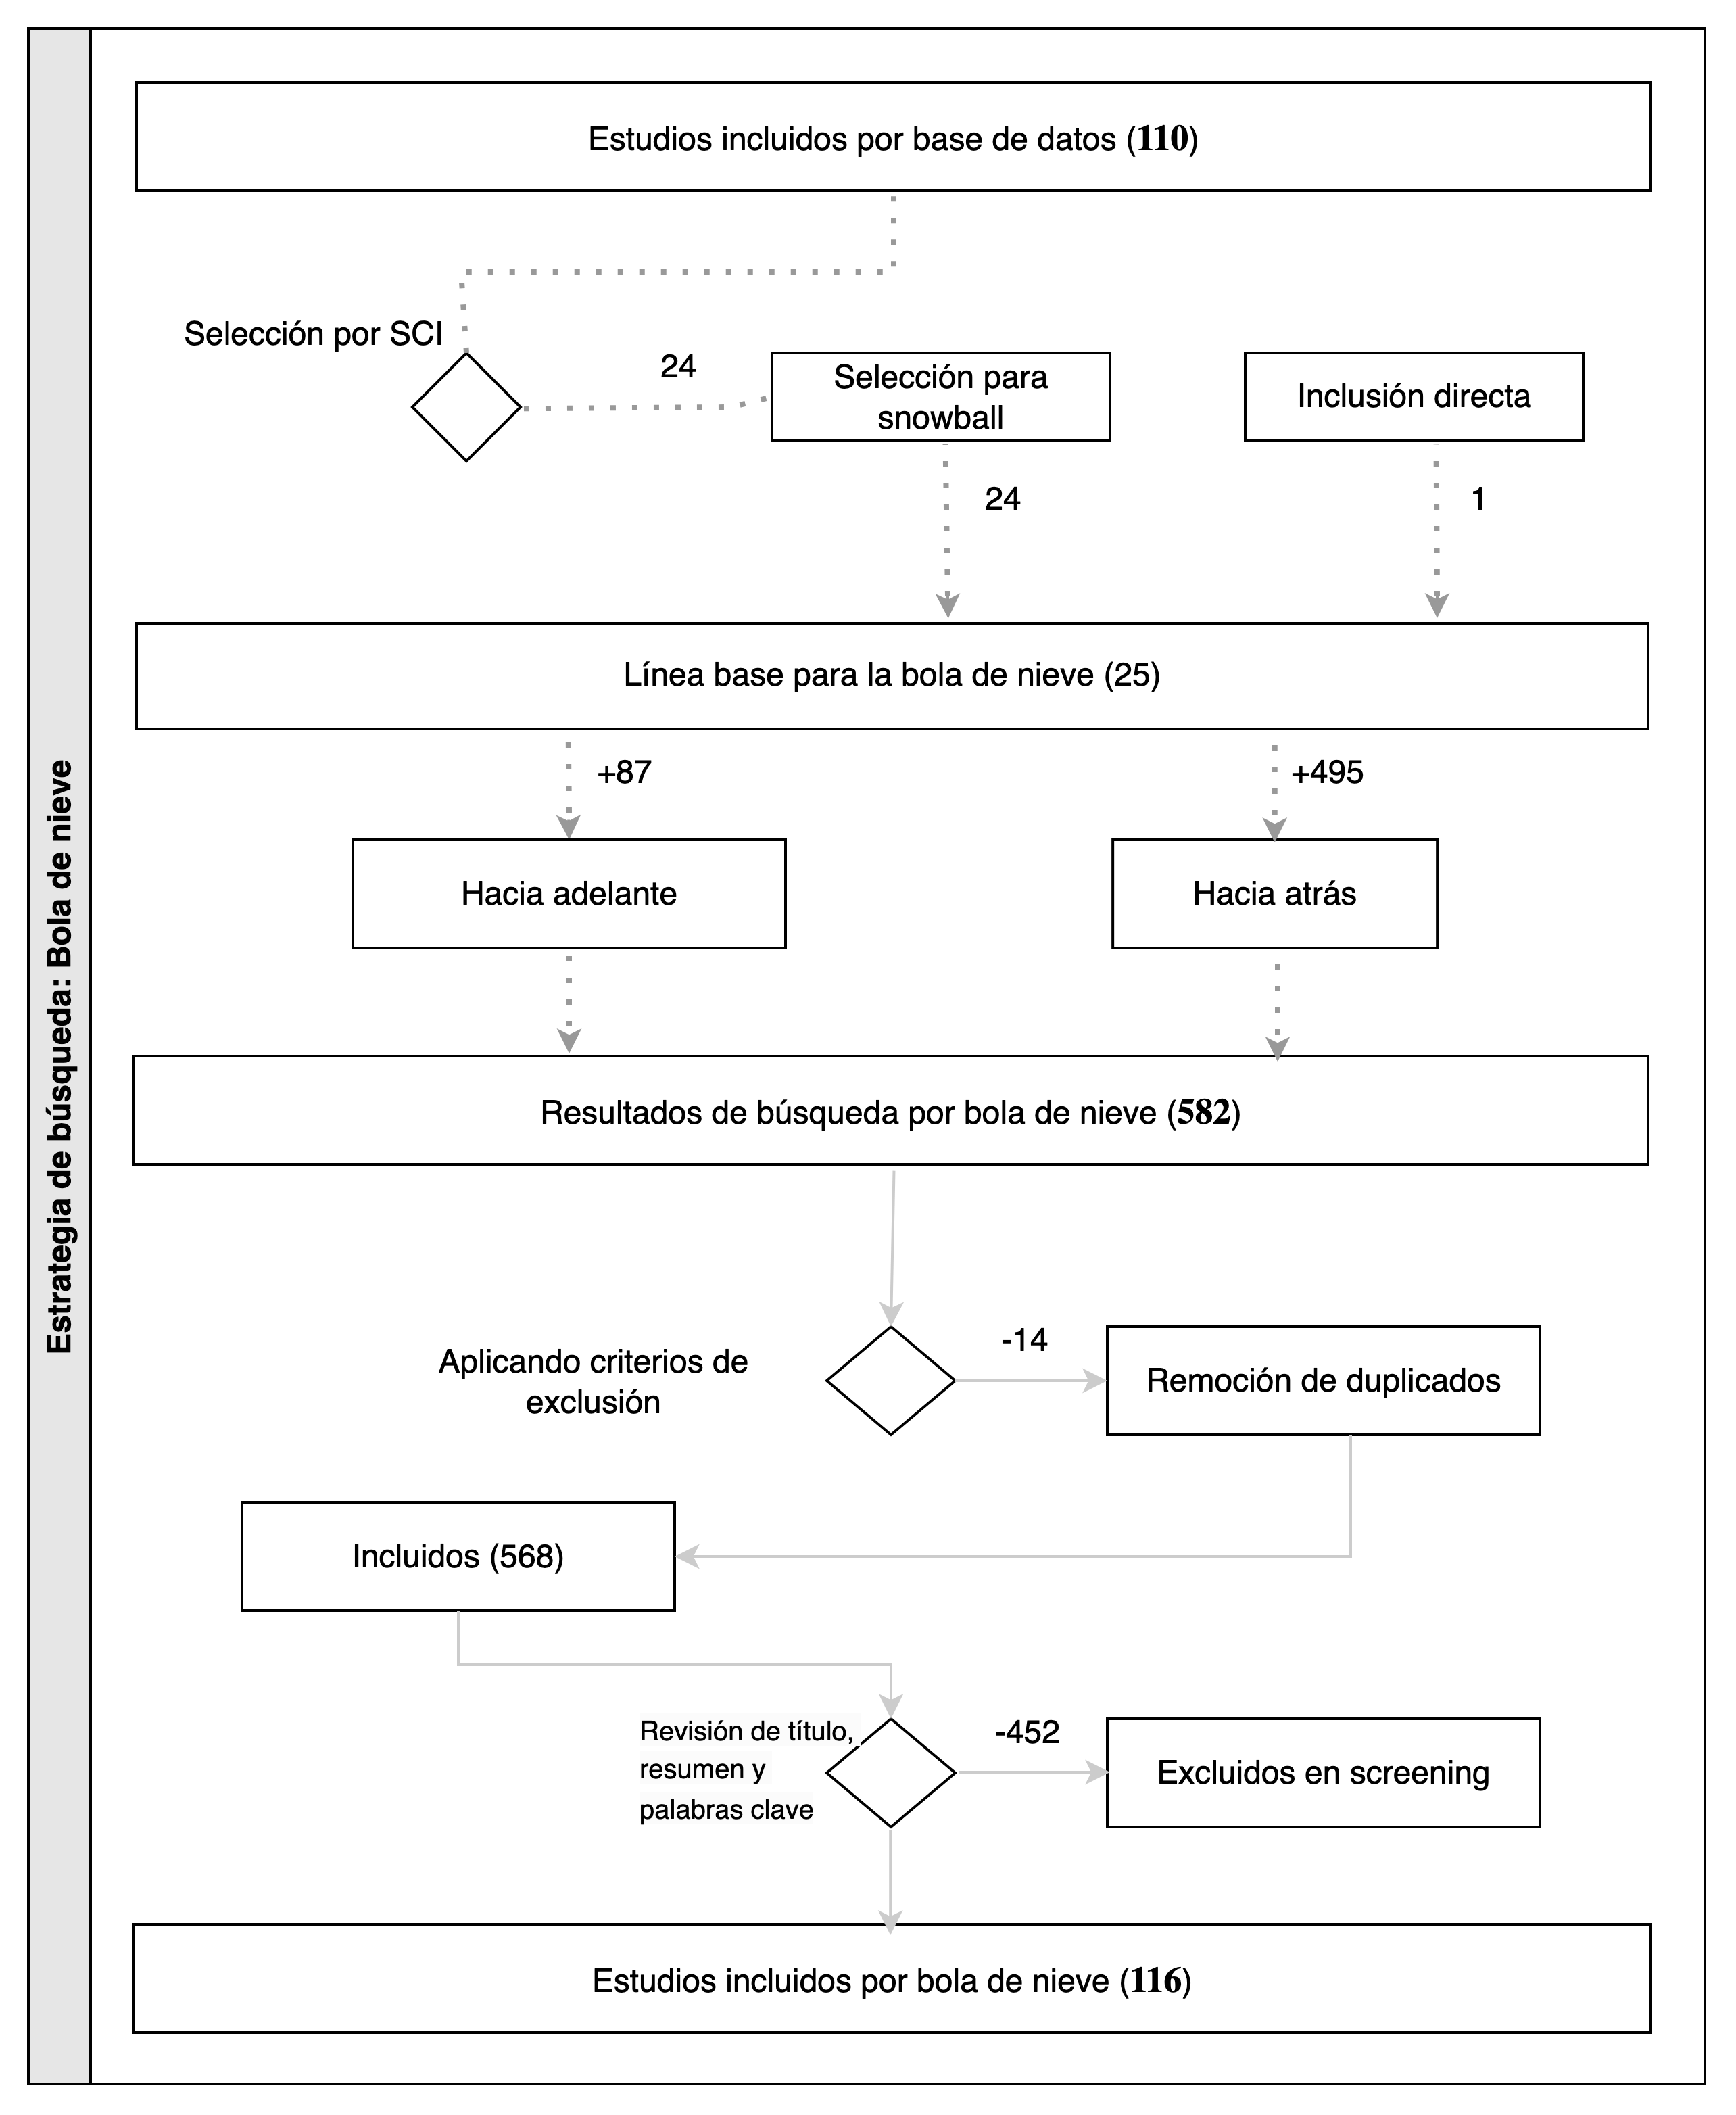
\includegraphics[scale=0.14]{tablas-images/cp2/diagrama-bola-nieve-busqueda.png}
    \caption{Diagrama de la búsqueda en bola de nieve}\label{tab:tabla-diagrama-bola-nieve-busqueda}
\end{table}

\section*{7 Identificación de estudios}
\addcontentsline{toc}{section}{Identificación de estudios}\label{sec:identificacionEstudios}

\subsection*{7.1 Artículos por año y métricas}
\addcontentsline{toc}{subsection}{Artículos por año y métricas}\label{subsec:articulosPorAnoYMetrica}
\begin{figure}[H]
    \centering
    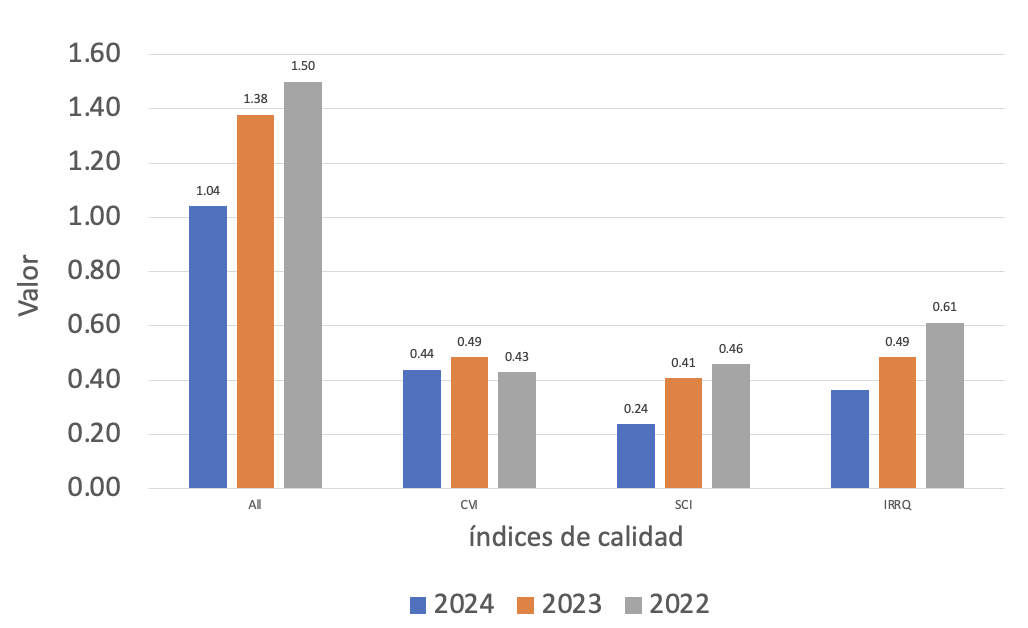
\includegraphics[width=\textwidth]{tablas-images/cp2/diagrama-articulos-ano-metrica.png}
    \caption{Artículos por métricas y año}\label{fig:diagrama-articulos-ano-metrica}
\end{figure}

\begin{figure}[H]
    \centering
    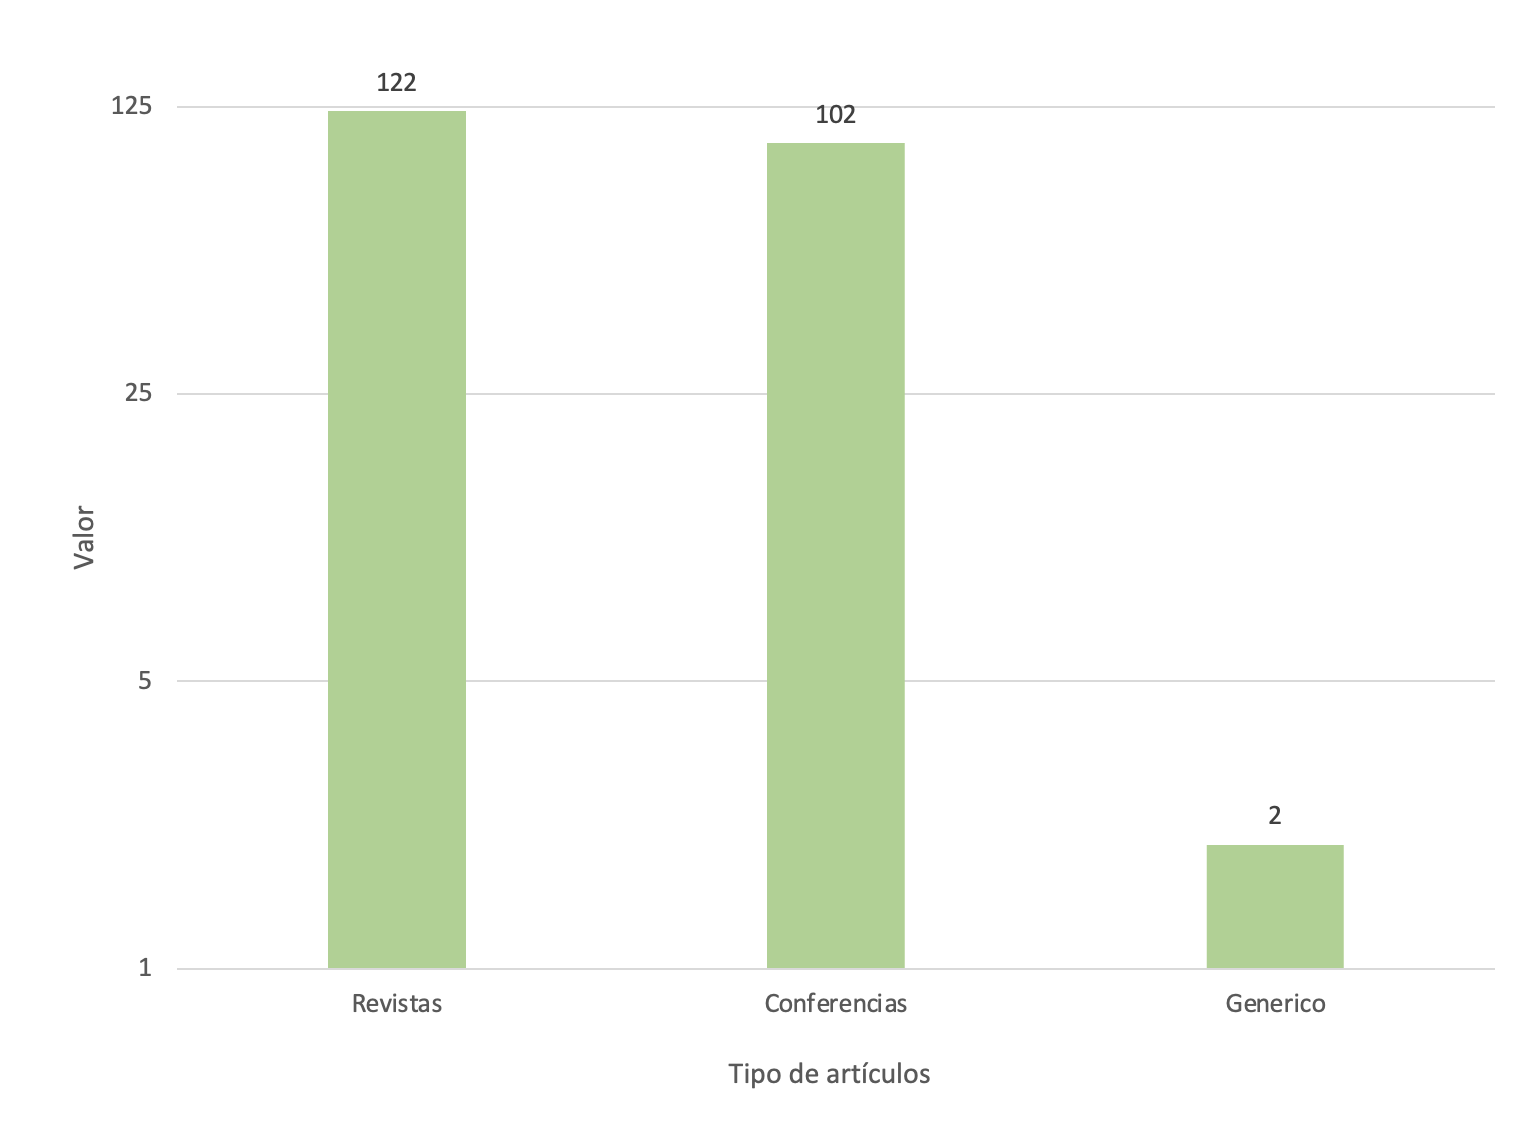
\includegraphics[width=\textwidth]{tablas-images/cp2/tipos-articulos.png}
    \caption{Artículos por tipo}\label{fig:tipos-articulos}
\end{figure}

\begin{figure}[H]
    \centering
    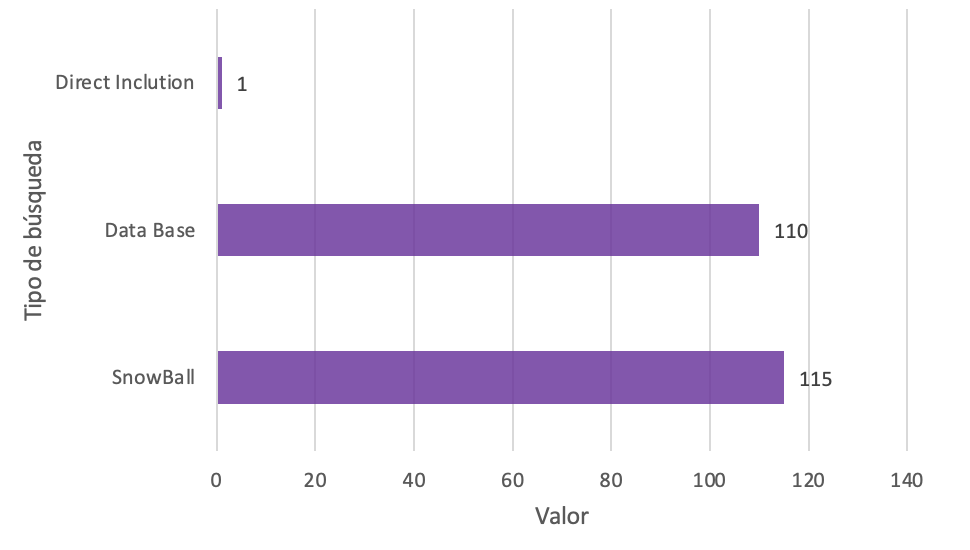
\includegraphics[width=\textwidth]{tablas-images/cp2/estrategia-busqueda-articulos.png}
    \caption{Estrategia de búsqueda de artículos}\label{fig:estrategia-busqueda-articulos}
\end{figure}

\begin{figure}[H]
    \centering
    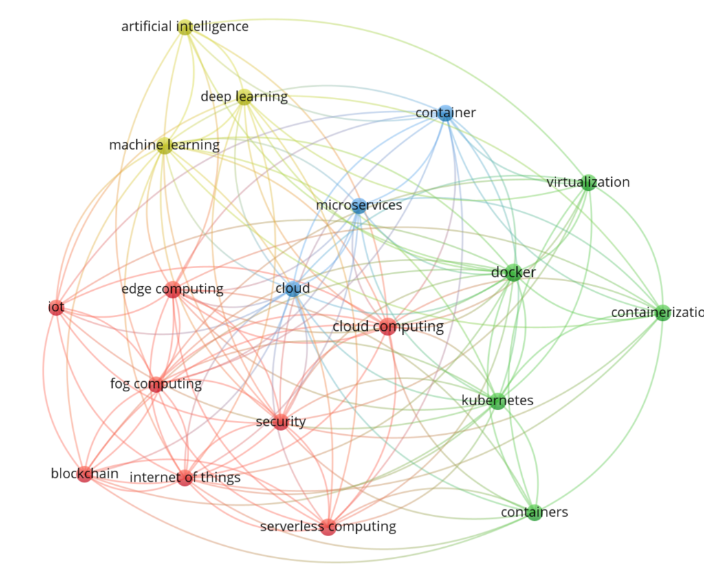
\includegraphics[width=\textwidth]{tablas-images/cp2/diagrama-red-busqueda.png}
    \caption{Diagrama de red de los artículos}\label{fig:diagrama-red-articulos}
\end{figure}

\section*{8 Información de la herramienta}
\addcontentsline{toc}{subsection}{Información de la herramienta}\label{subsec:informacionHerramienta}

\noindent
La herramienta utilizada para este proceso de revisión de la literatura fue \textbf{SMS-BUILDER}, la cual se encuentra disponible en \textit{Docker Hub}. El estudio realizado puede consultarse en el siguiente enlace:

\begin{center}
\href{https://sms-vbc.iti.grid.uniquindio.edu.co/}{\texttt{https://sms-vbc.iti.grid.uniquindio.edu.co/}}
\end{center}

\noindent
Adicionalmente, se implementaron procesos de respaldo como medida de seguridad. Estos \textit{backups} fueron almacenados en ubicaciones diferentes, siguiendo la estrategia de respaldo \textbf{3--2--1}.
